% !TEX root = ./sub-main.tex
\documentclass[main.tex]{subfiles}

\begin{document}
    \section{Sources of funding costs}
        In the context of an OTC derivatives dealer, 
        \textcite{Ruiz2013FVA} mentions some of the most likely sources of funding costs as
        either asymmetry in collateral agreements or the payment liabilities due to the contract itself.
        Both of these sources will be discussed in the following sections.
        As will be concluded, funding costs contribute to the cost of trading under imperfect CSA agreements 
        and trading derivatives whose market risk cannot be perfectly replicated.

    \subsection{Funding Costs from Asymmetrical Collateral Agreements}
    \label{sec:funding-asymmetric-collateral}
        Imbalance between the collateral schemes of an OTC deals and its market risk hedge
        is an origin of funding costs and the concern of this section.
        The conclusion will be that if a perfect market risk hedge exists, funding costs can be viewed 
        as a component of the cost of trading derivatives that are not subject to a perfect CSA agreement.

        After entering financial contracts with counterparties,
        a derivatives dealer will often enter into the opposite trades
        with the sole purpose of hedging market risk.
        Hedges will often be obtained in an exchange requiring full collateralization,
        since the dealer will be trading with other financial institutions.
        Therefore, when the collateralization scheme with the counterparty is imperfect, 
        its collateral cash flows will likely not match the collateral cash flows from the hedge.
        This source of funding costs is best introduced in its most extreme case, 
        where the dealer trades unsecured derivatives. 

        \begin{example}
        Consider the situation depicted in \cref{fig:funding-costs-unsecured-derivative}.
        The derivatives dealer is selling an unsecured OTC derivative to a counterparty,
        and the counterparty pays the upfront price of $\$\$\$$.
        The particular type of derivative is not too important, 
        but picture a derivative that can leave the dealer both negatively and positively exposed to the counterparty, 
        e.g. an interest rate swap.
        In order to avoid the market risk of the investment, 
        the dealer hedges the trade by performing the opposite, 
        perhaps synthetic, trade with an exchange,
        In this example, it is assumed that the upfront price of the derivative 
        matches exactly the upfront price of the market risk hedge.
        The exchange requires full collateralization;
        when the dealer has positive exposure to the counterparty, 
        she has negative exposure to the exchange and must post collateral. 
        When it has positive exposure to the counterparty it receives collateral.
        The collateral posted at the exchange is secured by the actual investment demanding the collateral;
        therefore, any collateral posted earns the \OIS/ rate at the receiver.
        The exchange could possibly charge a spread and pay less than the \OIS/ rate,
        but for simplicity assume that this is not the case.
        Assume also that the dealer's institution has no excess cash on its balance sheet, 
        such that any collateral that needs to be posted to the exchange 
        must be borrowed from the dealer's funding institution,
        in this case her funding desk. 
        This funding is unsecured and the funding desk charges a spread, here denoted by S,
        more specifically the dealer pays the rate $\OIS/ + \text{S}$.

        The excess interest rate charged by the funding desk is exactly the source of the funding cost.
        If the dealer has positive exposure to the counterparty, collateral must be posted to the exchange.
        The dealer then earns \OIS/ from the posted collateral but pays $\OIS/ + \text{S}$ for funding;
        the difference, S, drives the funding cost.
        Alternatively, the exchange posts collateral to the dealer, for which she pays \OIS/.
        If rehypothecation is allowed, the dealer can retire debt and save the funding spread.
        In this case, S drives the funding benefit.
        \end{example}

        \begin{figure}
            \centering
            \resizebox{\textwidth}{!}{%
            \begin{tikzpicture}
                % !TEX root = ./test-graphics.tex

\tikzmath{
    \arrowyoffset = 7;
    \arrowcenteryoffset = 7;
    \toparrowyoffset = \arrowcenteryoffset + \arrowyoffset;
    \bottomarrowyoffset = \arrowcenteryoffset - \arrowyoffset;
    \arrowtoboxpadding = 5;
}
\coordinate (center) at (0,0);
\node (dealer) at (center) [
    draw,
    fill=white!80!gray,
    very thick,
    minimum width=3cm,
    minimum height=2cm,
    align=center,
    rounded corners=.50cm,
] {Derivatives\\dealer};

\node (counterparty) at ($(dealer.west) + (-5, 0)$) [
    draw,
    very thick,
    minimum width=3cm,
    minimum height=2cm
] {Counterparty};

\node (exchange) at ($(dealer.east) + (5, 0)$) [
    draw,
    dashed,
    very thick,
    minimum width=3cm,
    minimum height=2cm,
] {Exchange};

\node (funding) at ($(dealer.south) + (0, -4)$) [
    draw,
    very thick,
    minimum width=3cm,
    minimum height=2cm,
] {Prime broker};

% Dealer - Counterparty relations
\draw[->, thick] 
    ([yshift=\bottomarrowyoffset pt, xshift=-\arrowtoboxpadding pt]dealer.south west) -- 
    ([yshift=\bottomarrowyoffset pt, xshift= \arrowtoboxpadding pt]counterparty.south east)
    node[near start, fill=white, inner sep=0pt] {
        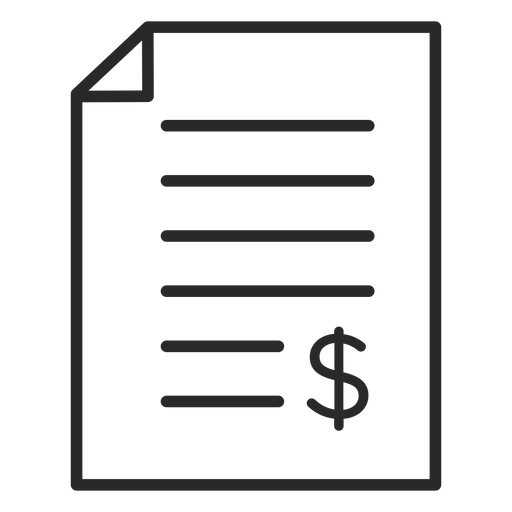
\includegraphics[width=0.60cm]{\graphicsfolder/source-of-funding-costs/contract}
    };
\draw[<-, thick] 
    ([yshift=\toparrowyoffset pt, xshift=-\arrowtoboxpadding pt]dealer.south west) -- 
    ([yshift=\toparrowyoffset pt, xshift= \arrowtoboxpadding pt]counterparty.south east)
    node[near end, fill=white, inner sep=2pt] {
        \$\$\$
    };

% Dealer - Exchange relations
\draw[<-, thick] 
    ([yshift=\bottomarrowyoffset, xshift= \arrowtoboxpadding pt]dealer.south east) -- 
    ([yshift=\bottomarrowyoffset, xshift=-\arrowtoboxpadding pt]exchange.south west)
    node[near end, fill=white, inner sep=0pt] {
        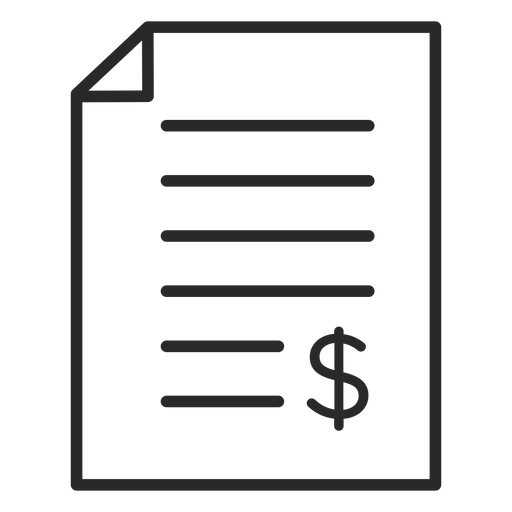
\includegraphics[width=0.60cm]{\graphicsfolder/source-of-funding-costs/contract}
    };
\draw[->, thick] 
    ([yshift=\toparrowyoffset, xshift= \arrowtoboxpadding pt]dealer.south east) -- 
    ([yshift=\toparrowyoffset, xshift=-\arrowtoboxpadding pt]exchange.south west)
    node[near start, fill=white, inner sep=2pt] {
        \$\$\$
    };

\draw[<->, thick, draw=blue] 
    ([yshift=-\bottomarrowyoffset, xshift= \arrowtoboxpadding pt]dealer.north east) -- 
    ([yshift=-\bottomarrowyoffset, xshift=-\arrowtoboxpadding pt]exchange.north west)
    node [pos=0.4, fill=white, inner sep=0pt] {
        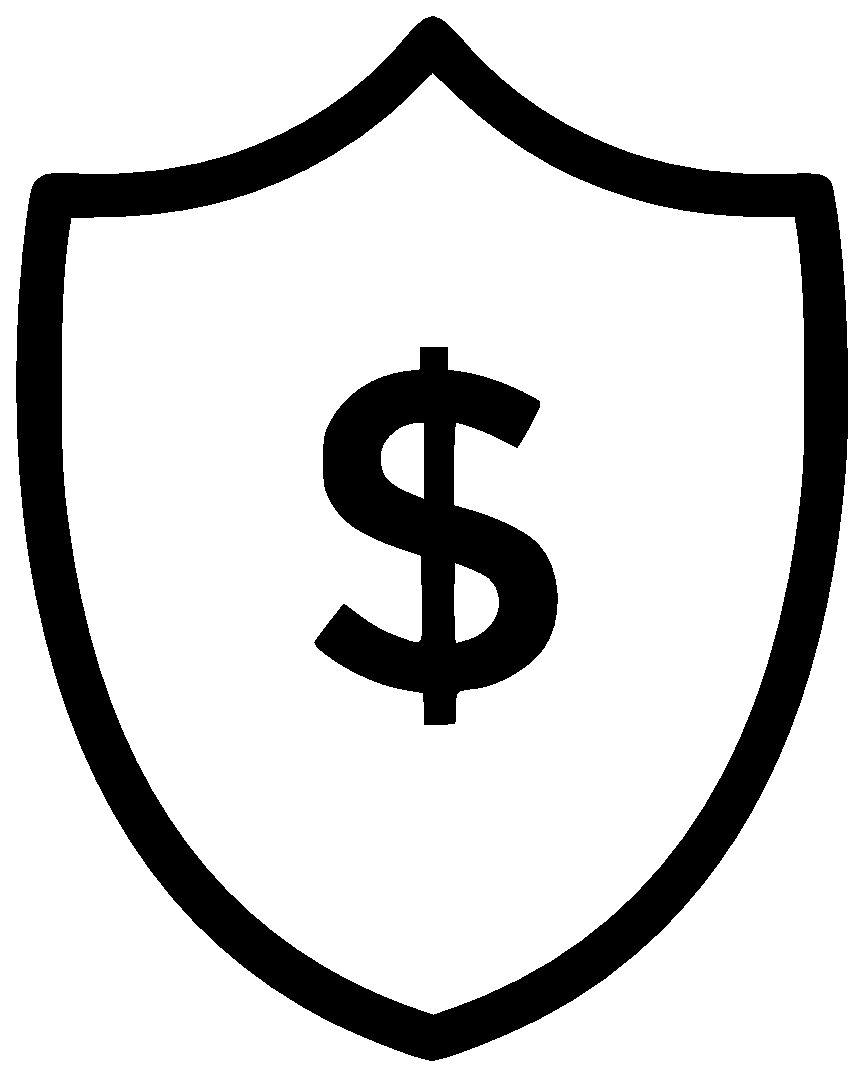
\includegraphics[width=0.65cm]{\graphicsfolder/source-of-funding-costs/collateral}
    };
\draw[<->, thick, draw=red] 
    ([yshift=-\toparrowyoffset, xshift= \arrowtoboxpadding pt]dealer.north east) -- 
    ([yshift=-\toparrowyoffset, xshift=-\arrowtoboxpadding pt]exchange.north west)
    node [pos=0.6, fill=white, inner xsep=2pt, inner ysep=0] {
        OIS
    };

% Dealer - Funding relations
\draw[<->, thick, draw=blue]
    ([xshift=-\arrowyoffset, yshift=-\arrowtoboxpadding]dealer.south) --
    ([xshift=-\arrowyoffset, yshift= \arrowtoboxpadding]funding.north)
    node[midway, fill=white, inner xsep=2pt, inner ysep=0, align=center, rotate=90] {
        Funding
    };
\draw[<->, thick, draw=red]
    ([xshift=\arrowyoffset, yshift=-\arrowtoboxpadding]dealer.south) --
    ([xshift=\arrowyoffset, yshift= \arrowtoboxpadding]funding.north)
    node[midway, fill=white, inner xsep=2pt, inner ysep=0, align=center, rotate=90] {
        OIS + S
    };
            \end{tikzpicture}        
            }   
            \caption{Illustration of funding costs from an unsecured OTC derivative.}
            \label{fig:funding-costs-unsecured-derivative}
        \end{figure}

        As mentioned, trading unsecured derivatives is the most extreme case,
        since any collateral call will lead to a funding surplus or deficit 
        and therefore, respectively, a funding benefit or cost.
        The funding cost can be reduced if the dealer has in place 
        a CSA agreement allowing rehypothecation with the counterparty.
        This would allow collateral to flow from the exchange to the counterparty, 
        or the opposite direction;
        therefore, collateral postings from one party could, partly or fully, 
        cover collateral needs from the other party.

        \begin{example}
        Consider the example illustrated in \cref{fig:funding-costs-secured-derivative}.
        Again, the dealer sells a derivative to her counterparty;
        however, in this case, the two parties are trading under a CSA agreement, 
        such that the trade is secured by collateralization.
        The posting of collateral by the counterparty reduces the credit risk of the dealer,
        but she still faces the market risk from the derivative;
        hence, she creates a market risk hedge at the exchange.
        
        Assume a perfect hedge, such that any market risk exposure to the counterparty 
        is exactly offset by the opposite exposure to the exchange.
        Whenever the dealer calls for collateral from the counterparty,
        she can expect a call for collateral from the exchange.
        Since rehypothecation is allowed,
        the collateral posted by the counterparty can be passed on to the exchange.
        To a certain extent, this reduces the dealer's need for borrowing unsecured funds from the funding desk
        and ultimately reduces her funding costs.
        However, funding costs are possibly still present as
        the collateral agreement with the counterparty is likely weaker than that with the exchange. 
        This is depicted in \cref{fig:funding-costs-secured-derivative} 
        by the shield on the counterparty side being smaller than the shield on the exchange side.
        The asymmetry has the implications that 
        collateral posted by the counterparty might only partly cover collateral calls from the exchange 
        and collateral posted by the exchange will more than cover collateral calls from the counterparty.

        The former requires the dealer to finance the difference and generates a funding cost.
        The latter provides a funding benefit.
        \end{example}

        \begin{figure}
            \centering
            \resizebox{\textwidth}{!}{%
            \begin{tikzpicture}
                % !TEX root = ./test-graphics.tex

% !TEX root = ./test-graphics.tex

\tikzmath{
    \arrowyoffset = 7;
    \arrowcenteryoffset = 7;
    \toparrowyoffset = \arrowcenteryoffset + \arrowyoffset;
    \bottomarrowyoffset = \arrowcenteryoffset - \arrowyoffset;
    \arrowtoboxpadding = 5;
}
\coordinate (center) at (0,0);
\node (dealer) at (center) [
    draw,
    fill=white!80!gray,
    very thick,
    minimum width=3cm,
    minimum height=2cm,
    align=center,
    rounded corners=.50cm,
] {Derivatives\\dealer};

\node (counterparty) at ($(dealer.west) + (-5, 0)$) [
    draw,
    very thick,
    minimum width=3cm,
    minimum height=2cm
] {Counterparty};

\node (exchange) at ($(dealer.east) + (5, 0)$) [
    draw,
    dashed,
    very thick,
    minimum width=3cm,
    minimum height=2cm,
] {Exchange};

\node (funding) at ($(dealer.south) + (0, -4)$) [
    draw,
    very thick,
    minimum width=3cm,
    minimum height=2cm,
] {Prime broker};

% Dealer - Counterparty relations
\draw[->, thick] 
    ([yshift=\bottomarrowyoffset pt, xshift=-\arrowtoboxpadding pt]dealer.south west) -- 
    ([yshift=\bottomarrowyoffset pt, xshift= \arrowtoboxpadding pt]counterparty.south east)
    node[near start, fill=white, inner sep=0pt] {
        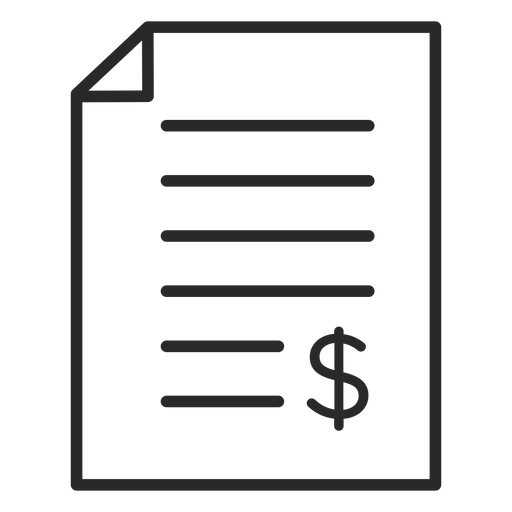
\includegraphics[width=0.60cm]{\graphicsfolder/source-of-funding-costs/contract}
    };
\draw[<-, thick] 
    ([yshift=\toparrowyoffset pt, xshift=-\arrowtoboxpadding pt]dealer.south west) -- 
    ([yshift=\toparrowyoffset pt, xshift= \arrowtoboxpadding pt]counterparty.south east)
    node[near end, fill=white, inner sep=2pt] {
        \$\$\$
    };

% Dealer - Exchange relations
\draw[<-, thick] 
    ([yshift=\bottomarrowyoffset, xshift= \arrowtoboxpadding pt]dealer.south east) -- 
    ([yshift=\bottomarrowyoffset, xshift=-\arrowtoboxpadding pt]exchange.south west)
    node[near end, fill=white, inner sep=0pt] {
        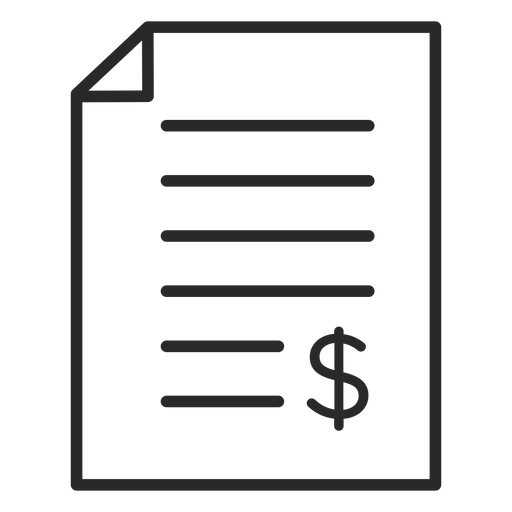
\includegraphics[width=0.60cm]{\graphicsfolder/source-of-funding-costs/contract}
    };
\draw[->, thick] 
    ([yshift=\toparrowyoffset, xshift= \arrowtoboxpadding pt]dealer.south east) -- 
    ([yshift=\toparrowyoffset, xshift=-\arrowtoboxpadding pt]exchange.south west)
    node[near start, fill=white, inner sep=2pt] {
        \$\$\$
    };

\draw[<->, thick, draw=blue] 
    ([yshift=-\bottomarrowyoffset, xshift= \arrowtoboxpadding pt]dealer.north east) -- 
    ([yshift=-\bottomarrowyoffset, xshift=-\arrowtoboxpadding pt]exchange.north west)
    node [pos=0.4, fill=white, inner sep=0pt] {
        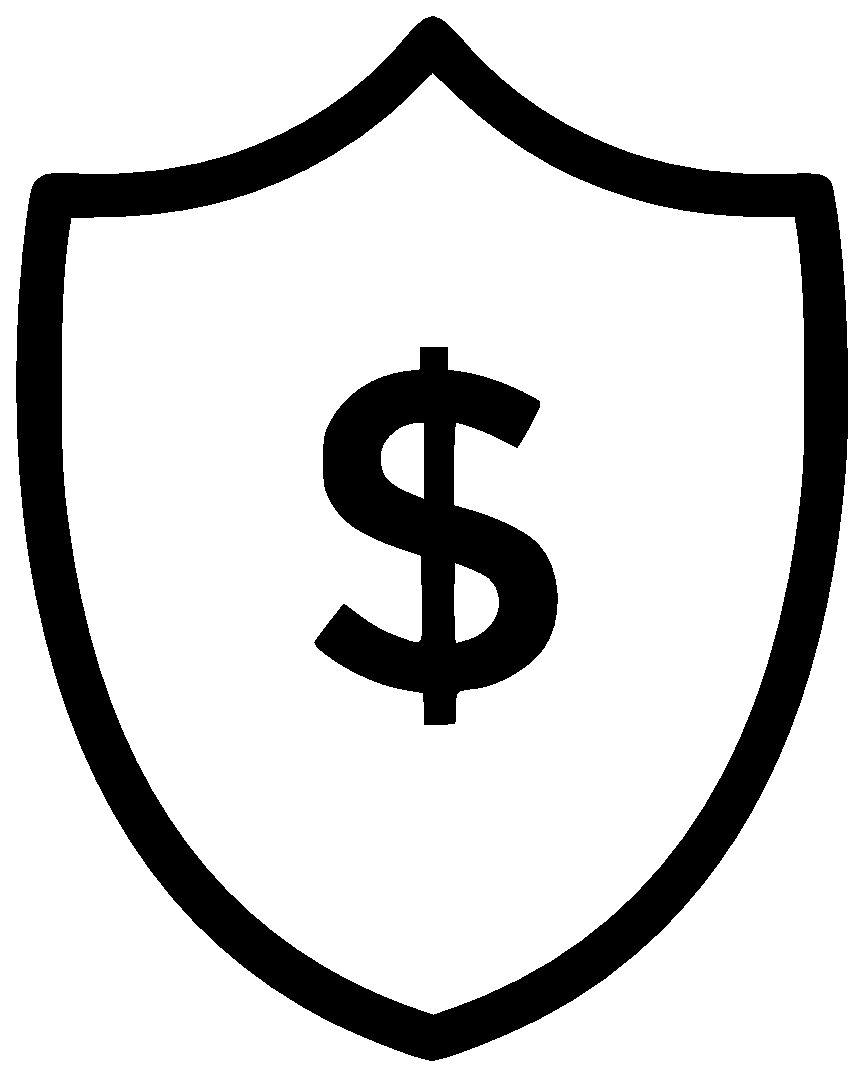
\includegraphics[width=0.65cm]{\graphicsfolder/source-of-funding-costs/collateral}
    };
\draw[<->, thick, draw=red] 
    ([yshift=-\toparrowyoffset, xshift= \arrowtoboxpadding pt]dealer.north east) -- 
    ([yshift=-\toparrowyoffset, xshift=-\arrowtoboxpadding pt]exchange.north west)
    node [pos=0.6, fill=white, inner xsep=2pt, inner ysep=0] {
        OIS
    };

% Dealer - Funding relations
\draw[<->, thick, draw=blue]
    ([xshift=-\arrowyoffset, yshift=-\arrowtoboxpadding]dealer.south) --
    ([xshift=-\arrowyoffset, yshift= \arrowtoboxpadding]funding.north)
    node[midway, fill=white, inner xsep=2pt, inner ysep=0, align=center, rotate=90] {
        Funding
    };
\draw[<->, thick, draw=red]
    ([xshift=\arrowyoffset, yshift=-\arrowtoboxpadding]dealer.south) --
    ([xshift=\arrowyoffset, yshift= \arrowtoboxpadding]funding.north)
    node[midway, fill=white, inner xsep=2pt, inner ysep=0, align=center, rotate=90] {
        OIS + S
    };

\draw[<->, thick, draw=fundingcolor] 
    ([yshift=-\bottomarrowyoffset, xshift=-\arrowtoboxpadding pt]dealer.north west) -- 
    ([yshift=-\bottomarrowyoffset, xshift= \arrowtoboxpadding pt]counterparty.north east)
    node (collateral) [pos=0.6, fill=white, inner sep=0pt] {
        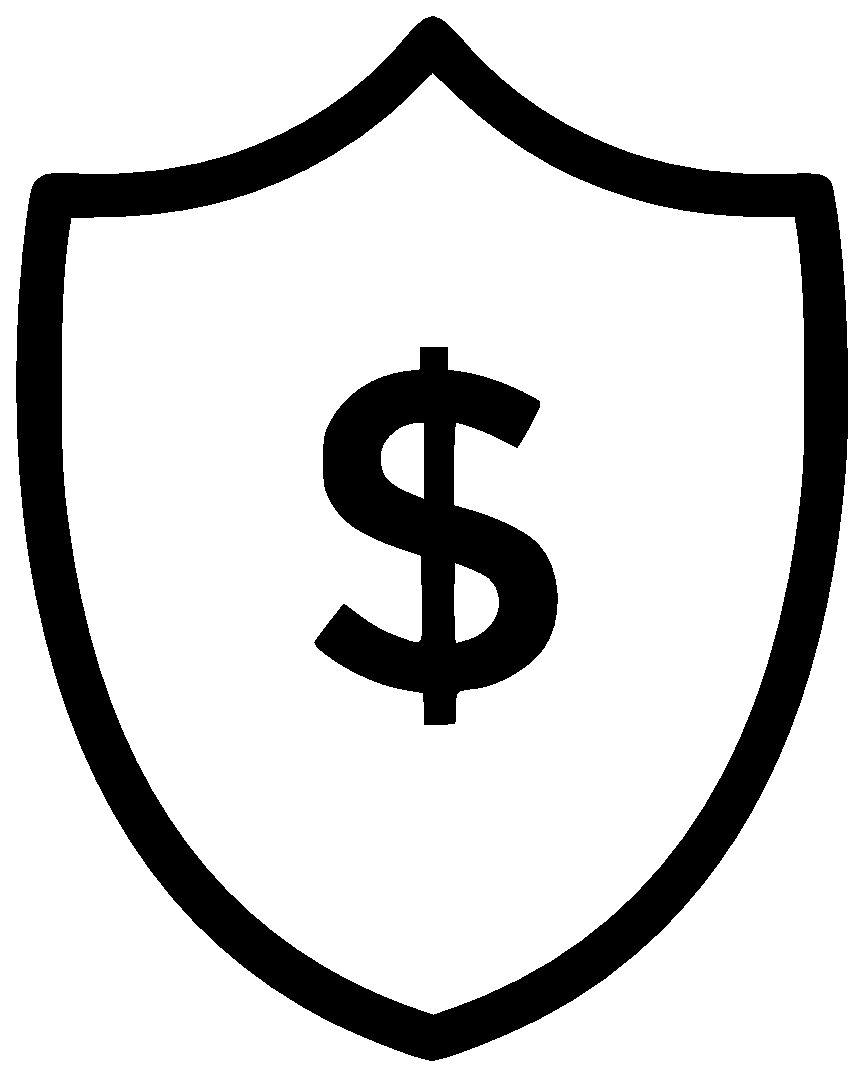
\includegraphics[width=0.40cm]{\graphicsfolder/source-of-funding-costs/collateral}
    };


\draw[<->, thick, draw=ratecolor] 
    ([yshift=-\toparrowyoffset, xshift=-\arrowtoboxpadding pt]dealer.north west) -- 
    ([yshift=-\toparrowyoffset, xshift= \arrowtoboxpadding pt]counterparty.north east)
    node [pos=0.4, fill=white, inner xsep=2pt, inner ysep=0] {
        OIS
    };
            \end{tikzpicture}        
            }   
            \caption{Illustration of funding costs from a secured OTC derivative.}
            \label{fig:funding-costs-secured-derivative}
        \end{figure}

        The differences between the CSA agreements, leading to the situation described above, could vary. 
        To mention a few, the CSA agreement with the counterparty might have higher exposure thresholds, 
        higher minimum transfer amounts, or lower frequency of margin calls.
        All of these differences lead the collateral cash flows to and from the exchange 
        to be at least as high as the cash flows to and from the counterparty. 
        In case the two collateral agreements are identical, the funding cost will be eliminated, 
        since the collateral received from the counterparty will completely suffice as collateral posted to the exchange.        

        To further grasp how unaligned collateralization schemes can lead to cash shortfalls or surpluses, 
        consider the example drawn by \cref{fig:funding-costs-asymmetrical-csa}.
        This example displays the possible implications of hedging a secured derivative
        with a trade that calls for collateral more frequently.

        \begin{example}
        The same dealer as previously trades an interest rate swap with a counterparty with whom a CSA is agreed upon. 
        The value of the dealer's part of the contract is drawn as a function of time 
        by the \textcolor{wtf-blue}{blue line} with dots.
        To hedge the market risk, the dealer enters into the opposite trade with an exchange.
        The market risk is perfectly hedged, and the value of the dealers contract is therefore
        equal to the dealer's contract with the counterparty but with the signs flipped.
        This value is indicated by the \textcolor{wtf-orange}{orange line}.
        For simplicity, both swaps can take only one of five values; $+\$$, $+\$\$$, $0$, $-\$$, and $-\$\$$.
        Both swaps are secured by CSA agreements allowing rehypothecation 
        and with no exposure thresholds or minimum transfer amounts.
        For the trade with the exchange, collateral calls can be submitted every time period;
        however, for the trade with the counterparty, collateral calls can only be submitted every second time period.
        These agreements lead to the collateral postings reported in the second row of the figure.
        Negative amounts are posted by the dealer, while positive amounts are posted to the dealer 
        from the corresponding entity.
        Each period, the exchange considers the current mark-to-market and its collateral balance with the dealer
        and either submits a collateral call, posts collateral, 
        or does nothing if the mark-to-market is unchanged since the last collateral posting.
        The same goes for the counterparty, except, only every second period.

        In periods where collateral can be posted for both trades, 
        the collateral posted by one trade will completely cover the collateral call from the other;
        hence, the dealer will neither have an excess nor a surplus of funds.
        However, in period 1, when the exchange calls for collateral,
        the counterparty is not obliged to post collateral to the dealer. 
        If the dealer does not have excess cash, 
        she will have to obtain the funding from its funding desk
        and therefore pay the unsecured borrowing rate of $\OIS/ + S$. 
        This debt can only be repaid in period 2 when the counterparty posts collateral.
        The asymmetry of the collateral cash flows in period 2
        is thus a contributor to the funding costs of the derivative.

        In period 5 the situation is the opposite.
        The exchange posts collateral to the dealer, 
        but, even though the counterparty trade is marked-to-market lower than in period 4,
        the counterparty cannot submit a collateral call. 
        The dealer is therefore in excess of funding,
        which she can pass on to her funding desk.
        The funding desk can rehypothecate the collateral
        by passing it onto traders with a shortfall of collateral.
        The collateral shortfalls would otherwise have had to be covered by borrowing funds 
        from the funding institution and the dealer is thereby saving the unsecured borrowing rate of $\OIS/ + S$.
        The asymmetry in period 5 is therefore a funding benefit to the dealer
        since the excess collateral have reduced her institution's financing needs elsewhere.
        While this example is concerned with difference in frequency of collateral calls,
        examples with difference in exposure thresholds or higher minimum transfer amounts 
        would convey the same message.
        When there is asymmetry in the collateral cash flows the dealer must provide or receive funding,
        which generates funding costs or benefits.
        \end{example}

        \begin{figure}
            \centering
            \resizebox{\textwidth}{!}{%
            \begin{tikzpicture}
                % !TEX root = ./test-graphics.tex

\colorlet{exchangecolor}{-red!50!yellow!75}
\colorlet{counterpartycolor}{red!50!yellow!75}
\colorlet{fundingcolor}{-red!75}
\colorlet{ratecolor}{red!75}

\matrix [
    matrix of nodes,
    nodes = {
        minimum width = 1.5cm,
        minimum height = 0.65cm
    },
    nodes in empty cells,
    column 1/.append style = {nodes={minimum width=1.2cm}},
    column 2/.append style = {anchor=base east},
    row 6/.append style = {nodes={color=counterpartycolor, minimum height=1cm}},
    row 7/.append style = {nodes={color=exchangecolor, minimum height=1cm}},
] (value) {
    & Time & 0 & 1 & 2 & 3 & 4 & 5 & 6 & 7 \\
    \hline
    & &  &   &   &   &   &   &   &   \\
    & &  &   &   &   &   &   &   &   \\
    & &  &   &   &   &   &   &   &   \\
    & &  &   &   &   &   &   &   &   \\
    \hline
    & Exchange & $-\$$ & $-\$$ &       &   & $+\$$ & $+\$\$\$$ & $-\$$   &   \\
    & Counterparty & $+\$$ &   \textcolor{black}{$\boldsymbol{\times}$}    & $+\$$ & \textcolor{black}{$\boldsymbol{\times}$}  & $-\$$ &   \textcolor{black}{$\boldsymbol{\times}$}  & $-\$\$$ &  \textcolor{black}{$\boldsymbol{\times}$} \\
    \hline
    & Balance & 0     & \node (funding1-in) {$-\$$};      & \node (funding1-out) {0};     
    &       0 & 0     & \node (funding2-out) {$+\$\$\$$}; & \node (funding2-in) {0};  & 0 \\
};

\draw[dashed] ($(value-4-2.west)!0.5!(value-3-2.west)$) -- ($(value-4-10.east)!0.5!(value-3-10.east)$);
% \node () at ([xshift=0.25cm] $(value-4-10.east)!0.5!(value-3-10.east)$) {$0$};

\foreach \labl [count=\row from 2] in {$+\$\$$, $+\$$, $-\$$, $-\$\$$} {
    \node[anchor=east] () at ([xshift=0cm] value-\row-3.west) {\labl};
}
\node [align=center, rotate=90, anchor=north] () at ($(value-4-1.west)!0.5!(value-3-1.west)$) 
    {\textbf{Swap value} \\ \footnotesize to dealer};
\node [align=center, rotate=90, anchor=north] () at ($(value-7-1.west)!0.5!(value-6-1.west)$) 
    {\textbf{Collateral} \\ \footnotesize to dealer};

\foreach \from/\to [count=\col from 3] in {2/1, 1/1, 1/1, 1/2, 2/4, 4/3, 3/3} {
    \tikzmath{%
        \from = \from + 1;
        \to = \to + 1;
        \nextcol = \col + 1;
    };
    \pgfmathtruncatemacro{\from}{\from};
    \pgfmathtruncatemacro{\to}{\to};
    \pgfmathtruncatemacro{\nextcol}{\nextcol};
    \draw[exchangecolor] 
        plot[mark=*] (value-\from-\col.center) -- 
        plot[mark=*] (value-\to-\nextcol.center);
}
\draw[exchangecolor] (value-4-10.center) -- (value-4-10.east);

\foreach \from/\to [count=\col from 3] in {3/4, 4/4, 4/4, 4/3, 3/1, 1/2, 2/2} {
    \tikzmath{%
        \from = \from + 1;
        \to = \to + 1;
        \nextcol = \col + 1;
    };
    \pgfmathtruncatemacro{\from}{\from};
    \pgfmathtruncatemacro{\to}{\to};
    \pgfmathtruncatemacro{\nextcol}{\nextcol};
    \draw[counterpartycolor] 
        plot[mark=*] (value-\from-\col.center) -- 
        plot[mark=*] (value-\to-\nextcol.center);
}
\draw[counterpartycolor] (value-3-10.center) -- (value-3-10.east);

\tikzmath{%
    \fundingyshift=-3.5;
    \arrowxshift=7;
    \arrowtoboxpadding = 5;
}
\node [draw, thick] (funding-institution-1) at ([yshift=\fundingyshift cm] funding1-in) {Prime broker};
\draw [<-, draw=fundingcolor, thick] 
    ([xshift=-\arrowxshift pt, yshift=-\arrowtoboxpadding] funding1-in.south) -- ([xshift=-\arrowxshift pt, yshift=\arrowtoboxpadding] funding-institution-1.north)
    node[rotate=90, midway, fill=white] {Funding};
\draw [->, draw=ratecolor, thick] 
    ([xshift=\arrowxshift pt, yshift=-\arrowtoboxpadding] funding1-in.south) -- ([xshift=\arrowxshift pt, yshift=\arrowtoboxpadding] funding-institution-1.north)
    node[rotate=90, midway, fill=white] {OIS + S};

\node [draw, thick] (funding-institution-2) at ([yshift=\fundingyshift cm] funding2-out) {Prime broker};
\draw [->, draw=fundingcolor, thick] 
    ([xshift=-\arrowxshift pt, yshift=-\arrowtoboxpadding] funding2-out.south) -- ([xshift=-\arrowxshift pt, yshift=\arrowtoboxpadding] funding-institution-2.north)
    node[rotate=90, midway, fill=white] {Funding};
\draw [<-, draw=ratecolor, thick] 
    ([xshift=\arrowxshift pt, yshift=-\arrowtoboxpadding] funding2-out.south) -- ([xshift=\arrowxshift pt, yshift=\arrowtoboxpadding] funding-institution-2.north)
    node[rotate=90, midway, fill=white] {OIS + S};
            \end{tikzpicture}        
            }   
            \caption{
                Illustration of funding costs from an interest rate swap with asymmetrical collateral agreements.
                The exchange is obliged to submit collateral calls or post collateral every period,
                while the counterparty must only do that every second period.
            }
            \label{fig:funding-costs-asymmetrical-csa}
        \end{figure}

        These examples should display how a derivatives dealer might face funding costs,
        when the lack of perfect symmetry in collateral needs calls for unsecured funding.
        It might be argued that the funding costs could be eliminated by trading derivatives,
        whose replication can be operated by repurchase agreements. 
        Seemingly, buying the hedging strategy at repo should eliminate the need for unsecured financing
        and thus the funding costs. 
        However, even when repo market exists, hedging might require unsecured funding,
        which can be shown with an example by \textcite{Castagna2012FVA}.
        Consider a dealer buying a European call option, with the intention to hedge the market risk.
        To create the hedging strategy the dealer must short an amount of the underlying asset corresponding to the option Delta of the call option.
        If the underlying asset can be sold at repo the dealer will receive the repo rate.
        However, to pay the premium for the call option the dealer must borrow unsecured funds from her funding institution,
        paying again the funding spread. 

        This section has shown how asymmetrical collateralization schemes
        can lead to funding costs. 
        When trades and their hedges have identical CSA agreements, 
        the collateral cash flows can offset each other and there is no need for funding collateral.
        However, when the hedge has stronger collateralization than the trade itself,
        the cash flows will not always align, which creates cash surpluses and deficits;
        and therefore funding costs or benefits.
        
    \subsection{Funding costs from derivatives cash flows}
        The fact that the dealer does not have access to risk-free funding
        can imply further contributions to the funding costs, besides that from collateral financing.
        First, note that cash flows arising from a derivative must also be funded at a non-risk-free rate
        and that these cash flows can be used for netting other cash flows in the dealer's portfolio.
        The second point implies that with the existence of a perfect replication,
        the cash flows from a derivative can be completely offset by the hedging strategy,
        such that no additional funding is required and no funding costs are generated.

        In reality, replications of OTC derivatives are most often imperfect,
        such that there is no one-to-one correspondence in cash flows between the derivative and the hedge.
        Of course, the dealer might not even try to hedge a derivative directly,
        but rather let a netting set of cash flows offset each other. 
        The principle is the same whether the derivative cash flows are offset by an imperfect hedge
        or another different derivative;
        both are again sources of funding cost, which can be illustrated by the following examples.

        The treatment of derivative cash flows from a funding cost perspective 
        depends on the type of cash flow and the reason why it occurs,
        as not all entail funding costs for the same reason.

        \begin{example}
        Consider a firm buying a simple option, without the intention to hedge its market risk.
        Buying the option requires paying an upfront price to the counterparty,
        which would seemingly require financing;
        however, this is only a source of funding costs 
        if the firm and the counterparty do not have a CSA agreement in place.
        If both the firm and the counterparty are financial institutions, 
        they will most likely maintain a CSA agreement
        such that any upfront price paid will immediately be met by a collateral posting in the opposite direction.
        Hence, the funding need for the upfront price will be satisfied and the funding costs eliminated.
        If no CSA exists and no collateral is posted, the upfront will still create funding costs,
        while selling the option instead will decrease the funding needs and create a funding benefit.
        This is not to say that a CSA agreement will eliminate funding costs completely. 
        Hedging cash flows might also generate funding needs or surpluses, 
        e.g. if a dealer must apply leverage to properly hedge a positions 
        and pay the higher rates of leverage due to financing spreads.
        \end{example}

        Another source of funding costs materializes in the next example when the dealer applies an imperfect hedge.
        
        \begin{example}
        The dealer have entered into a 10 year OTC swap with semi-annual payments, 
        but for the replication the dealer is only able to obtain a 10 year swap with quarterly payments.
        As a result, the dealer will have a cash flow from the hedge every three months
        that does not correspond to the cash flow from the OTC derivative. 
        Both of these are examples of funding costs essentially stemming from the lack of perfect hedging.
        \end{example}

        Having established some possible sources of funding costs, 
        the discussion can move on to the debate about whether accounting for these is appropriate for derivatives pricing.

\end{document}
        